\section{Considerazioni generali}\label{considerazioniGenerali}
Questa sezione contiene delle considerazioni riguardanti il sito in generale o a elementi comuni a più pagine.

\subsection{Nome del sito}%Check
Il nome del sito, se scelto correttamente, aiuta l'utente a capire il contenuto del sito e gli permette di farsi un'idea dei contenuti che troverà. In questo caso il nome \siteName lascia facilmente intuire all'utente il tema del sito: \textit{fotografia}.

\subsection{Design}%Check
Il design del sito è semplice e comune a molti altri siti web, questo riduce lo sforzo computazionale da parte dell'utente che alla prima visita ha già un'idea riguardo a come è strutturata la pagina.
Lo schema dei colori (rosso, bianco e nero) garantisce un buon contrasto, rendendo possibile una corretta visualizzazione del testo anche a persone con disturbi visivi, inoltre i colori scelti non sono accecanti e rendono piacevole la navigazione.

\subsection{Navigazione}%Check
Lo spostamento tra le pagine del sito avviene principale mediante una barra di navigazione posta nella parte alta della pagina e che rimane visibile anche quando si scrolla, fornendo al visitatore la possibilità di passare da una sezione all'altra senza dover tornare all'inizio della pagina.
L'ingombro causato da questa barra è trascurabile dato la dimensione che risulta essere minima.\\
Le voci della barra di navigazione sono racchiuse in dei menù a tendina, questi menù sono stati progettati correttamente, infatti:
\begin{itemize}
\item Le voci sono facilmente cliccabili, è difficile selezionare una voce al posto di un'altra;
\item La voce sulla quale è posizionato il mouse viene colorata in modo diverso alle altre, facilitando la distinzione dalle altre;
\item Le varie tendine a scomparsa sono dotate di un timer di chiusura che ritarda la scomparsa delle tendina in modo da evitare le chiusure accidentali.
\end{itemize}
Tuttavia è presente il problema \textit{lost in navigation} in quanto manca una breadcrumbs che indichi all'utente il percorso fatto nella gerarchia del sito. Inoltre, il colore dei link già visitati non cambia, e è lo stesso usato per i link da visitare, lasciando così al visitatore il compito di ricordare quale zone del sito ha già visitato.
Sempre riguardo i link, non sono mai sottolineati, viene semplicemente usato del testo di colore diverso per evidenziarli, questo potrebbe portare difficoltà di consultazione a persone con disturbi visivi.

\subsubsection{Ricerca}%Check + Immagine
Nel sito è presente un tool che permette all'utente di effettuare una ricerca tra i vari articoli presenti nel sito, questo tool fornisce dei buoni risultati che vengono presentati al visitatore in modo analogo a come vengono visualizzati i vari articoli nella homepage, riducendo lo sforzo computazionale che l'utente deve compiere.

Anche se il tool di ricerca funziona correttamente, è presente un grave errore riguardo l'accesso alla casella di ricerca, infatti, a causa di un errore riguardante il codice del sito, la casella di ricerca viene visualizzata senza un colore di sfondo, rendendone difficile l'identificazione all'interno della pagina.

\begin{figure}[htpb]
\begin{center}

\includegraphics[width=0.8\textwidth]{immagini/erroreRicerca.png}
\caption{Box di ricerca del sito}
\label{errRicerca}
\end{center}
\end{figure}
\FloatBarrier

\subsection{Testo}%Check
Il testo presente nel sito è sempre facilmente leggibile, questo grazie al contrasto elevato (testo nero su sfondo bianco) e al font adottato, infatti, i vari testi del sito sono scritti con un font sans-serif.
Vengono inoltre rispettate le varie regole riguardo alla corretta impaginazione del testo: le righe sono di lunghezza limitata, tra i vari paragrafi sono presenti delle spaziature, utilizzo dei titolo per i paragrafi e così via.


\subsection{Pubblicità}%Check
Nelle varie pagine del sito sono presenti dei banner pubblicitari, sotto la barra di navigazione, all'inizio e alla fine di ogni articolo, cioè nei punti caldi della pagine aumentando la probabilità che l'utente li noti.\\
Il contenuto di queste pubblicità viene determinato dallo storico delle ricerche dell'utente\footnote{Viene utilizzato il servizio Google AdSense} fornendogli pubblicità mirate. Inoltre, queste pubblicità consistono solo in immagini o testo, evitando così di disturbare il visitatore.

\subsection{Pop up}%Check + Immagini
Nel sito sono presenti due pop up, uno che viene visualizzato solamente al primo accesso al sito e che invita il visitatore ad iscriversi subito alla newsletter via e-mail e un altro che viene visualizzato ogni volta che l'utente evidenzia del testo di un articolo.\\
Quest'ultima tipologia di pop up risulta essere estremamente fastidiosa, specialmente per le persone che tendono a selezionare con il cursore del mouse il testo che stanno leggendo.

\begin{figure}
\centering
\begin{subfigure}{.5\textwidth}
  \centering
  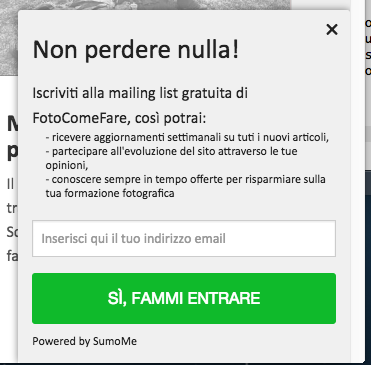
\includegraphics[width=.9\linewidth]{immagini/popUp2.png}
  \caption{Pop up per l'iscrizione alla newsletter}
  \label{fig:sub1}
\end{subfigure}%
\begin{subfigure}{.5\textwidth}
  \centering
  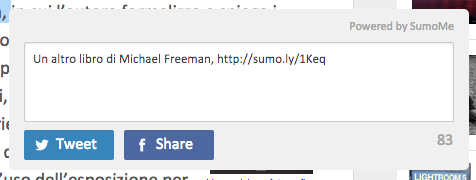
\includegraphics[width=.9\linewidth]{immagini/popUp1.png}
  \caption{Pop up che compare quando si seleziona del testo}
  \label{fig:sub2}
\end{subfigure}

\caption{Vari pop up presenti nel sito}
\label{popUp}
\end{figure}

\FloatBarrier

\subsection{Gestione del 404}%Check
L'errore 404 viene gestito in modo corretto, viene fornito al visitatore sia un messaggio che descrive il problema, sia la casella di ricerca per aiutarlo a trovare quello che stava cercando.